\documentclass[14pt,aspectratio=1610]{beamer}

\usepackage[brazil]{babel}
\usepackage[utf8]{inputenc}
%\UseRawInputEncoding
\usepackage[T1]{fontenc}
\usepackage{Sweave}
\usepackage{animate}
\usepackage{amsbsy}
\usepackage{amsfonts}
\usepackage{amsmath}
\usepackage{amssymb}
\usepackage{amsthm}
\usepackage[toc,page,title,titletoc]{appendix}
\usepackage[fixlanguage]{babelbib}
%\usepackage[pdftex]{color}
\usepackage{dsfont}
\usepackage{esvect}
\usepackage[labelfont=bf]{caption}
\usepackage{float}
\usepackage[Glenn]{fncychap}%Sonny %Conny %Lenny %Glenn %Renje %Bjarne %Bjornstrup
%\usepackage{geometry, calc, color, setspace}%
%\geometry{a4paper, headsep=1.0cm, footskip=1cm, lmargin=3cm, rmargin=2cm, tmargin=3cm, bmargin=2cm}
\usepackage{graphicx}
\usepackage{indentfirst}%Para indentar os parágrafos automáticamente
\usepackage{lipsum}
\usepackage{longtable}
\usepackage{mathtools}
\usepackage{listings}%Inserir codigo do R no latex
\usepackage{multirow}
\usepackage{multicol}
\usepackage{natbib}
\bibliographystyle{abbrvnat3}
\usepackage[figuresright]{rotating}
\usepackage{spalign}
%\usepackage{pgfpages}
\usepackage{pgfplots}
\usepackage{tikz}
\usepackage{color, colortbl}
\usepackage{ragged2e}%para justificar o texto dentro de algum ambiente
\definecolor{Gray}{gray}{0.9}
\definecolor{LightCyan}{rgb}{0.88,1,1}


\usepackage[all]{xy}
\usepackage{hyperref,bookmark}
\hypersetup{
  colorlinks=true,
  linkcolor=blue,
  citecolor=red,
  filecolor=blue,
  urlcolor=blue,
}

\usetheme{Madrid}
%\usecolortheme[RGB={193,0,0}]{structure}

%\setbeamertemplate{footline}[frame number]
%\setbeamertemplate{footline}[text line]{%
%  \parbox{\linewidth}{\vspace*{-8pt}\hfill\date{}\hfill\insertshortauthor\hfill\insertpagenumber}}
\beamertemplatenavigationsymbolsempty
\renewcommand{\vec}[1]{\mbox{\boldmath$#1$}}
\newtheorem{Teorema}{Teorema}
\newtheorem{Proposicao}{Proposição}
\newtheorem{Definicao}{Definição}
\newtheorem{Corolario}{Corolário}
\newtheorem{Demonstracao}{Demonstração}
\newcommand{\bx}{\ensuremath{\bar{x}}}
\newcommand{\Ho}{\ensuremath{H_{0}}}
\newcommand{\Hi}{\ensuremath{H_{1}}}
\everymath{\displaystyle}

\apptocmd{\frame}{}{\justifying}{} % Allow optional arguments after frame.

\title{MAF 105 - Iniciação à Estatística}
\author{Prof. Fernando de Souza Bastos}
\institute{Instituto de Ciências Exatas e Tecnológicas\texorpdfstring{\\ Universidade Federal de Viçosa}{}\texorpdfstring{\\ Campus UFV - Florestal}{}}
\date[\today]{}
\newcommand\mytext{Aula 1}
\newcommand\mytextt{Fernando de Souza Bastos}
\makeatletter
\setbeamertemplate{footline}
{
  \leavevmode%
  \hbox{%
  \begin{beamercolorbox}[wd=.333333\paperwidth,ht=2.25ex,dp=1ex,center]{author in head/foot}%
    \usebeamerfont{author in head/foot}\mytext
  \end{beamercolorbox}%
  \begin{beamercolorbox}[wd=.333333\paperwidth,ht=2.25ex,dp=1ex,center]{title in head/foot}%
    \usebeamerfont{title in head/foot}\mytextt
  \end{beamercolorbox}%
  % \begin{beamercolorbox}[wd=.333333\paperwidth,ht=2.25ex,dp=1ex,right]{date in head/foot}%
  %   \usebeamerfont{date in head/foot}\insertshortdate{}\hspace*{2em}
  %   \insertframenumber{} / \inserttotalframenumber\hspace*{2ex} 
  % \end{beamercolorbox}
  }%
  \vskip0pt%
}
\makeatother


\providecommand{\arcsin}{} \renewcommand{\arcsin}{\hspace{2pt}\textrm{arcsen}}
\providecommand{\sin}{} \renewcommand{\sin}{\hspace{2pt}\textrm{sen}}
%\newtheorem{Teorema}{Teorema}
%\newtheorem{Proposicao}{Proposição}
%\newtheorem{Definicao}{Definição}
%\newtheorem{Corolario}{Corolário}
%\newtheorem{Demonstracao}{Demonstração}

% Layout da pagina
\hypersetup{pdfpagelayout=SinglePage}
\begin{document}
\Sconcordance{concordance:Aula6.tex:Aula6.Rnw:%
1 1182 1}


\frame{\titlepage}

\begin{frame}{}
\frametitle{\bf Sumário}
\tableofcontents
\end{frame}

\section{Probabilidade Condicional e Independência}
\begin{frame}{}
\frametitle{}
\begin{block}{}
\justifying
Para dois eventos quaisquer $A$ e $B,$ sendo $P(B)>0,$ definimos a probabilidade
condicional de $A$ dado $B,$ como sendo 
\begin{align}\label{bayes}
P(A|B)=\dfrac{P(A\cap B)}{P(B)}
\end{align}
Assim, a probabilidade de $A$ muda após o evento $B$ ter acontecido. Isso porque o resultado de $A$ é uma das 
possibilidades de $B$ ou de $B^{c}.$ 
\end{block}
\end{frame}


\begin{frame}{}
\frametitle{Exemplo}
\begin{block}{}
\justifying
Considere-se um baralho de 52 cartas. A probabilidade de ao retirar uma
carta sair um rei é $4/52,$ ou $1/13.$ No entanto, se alguém retira uma
carta e nos diz que é uma figura, então a probabilidade de a carta retirada
ser um rei é $4/12=1/3,$ ou seja, $P(\textrm{sair um rei}|\textrm{sair uma
figura})=1/3.$
\end{block}
\end{frame}

\begin{frame}{}
\frametitle{Exemplo}
\begin{block}{}
\begin{columns}
        \column{5cm}
\begin{block}{}
\pgfdeclareimage[height=6cm,width=5cm]{ex1}{Figuras/ex1}
\pgfuseimage{ex1}
\end{block}
        \column{10cm}
Uma urna contém 10 bolas brancas e 10 bolas pretas. Retiro sucessivamente 2 bolas, sem reposição. Qual é a probabilidade de:
\begin{description}
\item[a)] Ambas pretas?\pause\\
$P(P_{1}\cap P_{2})=P(P_{1})\times P(P_{2}|P_{1})$
\item[b)]Segunda ser preta?\pause\\
$P(P_{2})=P[(P_{1}\cap P_{2})\cup (P_{2}\cap P_{2})]$
\end{description}
\end{columns}
\end{block}     
\end{frame}

\begin{frame}{}
\frametitle{}
\begin{block}{}
\begin{center}
\begin{tikzpicture}[grow=right]
\tikzstyle{level 1}=[sibling distance=3.5cm, level distance=2cm]
\tikzstyle{level 2}=[sibling distance=2cm, level distance=3cm]
\tikzstyle{arestas}=[rectangle, rounded corners=4pt, fill=white,font=\scriptsize]
 \node{}
  child{
      node{Branca}
    child{
      node{Branca}
      edge from parent
      node[arestas]{$\dfrac{9}{19}$}
    }
    child{
      node{Preta}
      edge from parent
      node[arestas]{$\dfrac{10}{19}$}
    }
  edge from parent
  node[arestas]{$\dfrac{1}{2}$}
  }
  child{
      node{Preta}
    child{
      node{Branca}
      edge from parent
      node[arestas]{$\dfrac{10}{19}$}
    }
    child{
      node{Preta}
      edge from parent
      node[arestas]{$\dfrac{9}{19}$}
    }
  edge from parent
  node[arestas]{$\dfrac{1}{2}$}
  };
\end{tikzpicture}
\end{center}
\end{block}
\end{frame}

\begin{frame}{}
\frametitle{}
\begin{block}{}
\begin{table}[H]
\begin{tabular}{c|c}
\hline
Resultados&Probabilidades\\
\hline
BB&$\dfrac{9 }{38}$\\
&\\
BP&$\dfrac{10}{38}$\\
&\\
PB&$\dfrac{10}{38}$\\
&\\
PP&$\dfrac{9 }{38}$\\
&\\
\hline
Total&1\\
\hline
\end{tabular}
\end{table}
\end{block}
\end{frame}

\begin{frame}{}
\frametitle{}
\begin{block}{}
\begin{center}
\begin{figure}
\caption{Com reposição}
\begin{tikzpicture}[grow=right]
\tikzstyle{level 1}=[sibling distance=3.5cm, level distance=2cm]
\tikzstyle{level 2}=[sibling distance=2cm, level distance=3cm]
\tikzstyle{arestas}=[rectangle, rounded corners=4pt, fill=white,font=\scriptsize]
 \node{}
  child{
      node{Branca}
    child{
      node{Branca}
      edge from parent
      node[arestas]{$\dfrac{1}{2}$}
    }
    child{
      node{Preta}
      edge from parent
      node[arestas]{$\dfrac{1}{2}$}
    }
  edge from parent
  node[arestas]{$\dfrac{1}{2}$}
  }
  child{
      node{Preta}
    child{
      node{Branca}
      edge from parent
      node[arestas]{$\dfrac{1}{2}$}
    }
    child{
      node{Preta}
      edge from parent
      node[arestas]{$\dfrac{1}{2}$}
    }
  edge from parent
  node[arestas]{$\dfrac{1}{2}$}
  };
\end{tikzpicture}
\end{figure}
\end{center}
\end{block}
\end{frame}

\begin{frame}{}
\frametitle{}
\begin{block}{}
\begin{table}[H]
\begin{tabular}{c|c}
\hline
Resultados&Probabilidades\\
\hline
BB&$\dfrac{1}{4}$\\
&\\
BP&$\dfrac{1}{4}$\\
&\\
PB&$\dfrac{1}{4}$\\
&\\
PP&$\dfrac{1}{4}$\\
&\\
\hline
Total&1\\
\hline
\end{tabular}
\end{table}
\end{block}
\end{frame}

\begin{frame}{}
\frametitle{}
\begin{block}{}
\justifying
Observem que, neste segundo caso, $P(B_{2}|B_{1})=P(B_{2})=\dfrac{1}{2}.$ Ou seja, 
$$P(A|B)=P(A)\ \textrm{ou}\ P(B|A)=P(B).$$ Nesse caso, dizemos que o evento $A$ independe do evento $B$ e, usando (\ref{bayes}), temos que 
\begin{align}\label{ind}
P(A\cap B)=P(A)P(B)
\end{align}
É fácil ver que se $A$ independe de $B,$ então $B$ independe de $A.$ A fórmula acima pode ser tomada como definição de independência entre dois eventos, ou seja, $A$ e $B$ são independentes se, e somente se, (\ref{ind}) for válida.

\end{block}
\end{frame}

\begin{frame}{}
\frametitle{}
\begin{block}{}
\justifying
Considere ainda a urna dos exemplos anteriores, mas vamos fazer três extrações sem reposição. Indiquemos por $P_{i}$ ou $B_{i}$ a obtenção de bola preta ou branca
na i-ésima extração, respectivamente, $i = 1, 2, 3.$
\end{block}
\end{frame}

\begin{frame}{}
\frametitle{}
\begin{block}{}
\begin{center}
\begin{tikzpicture}[grow=right]
\tikzstyle{level 1}=[sibling distance=4cm, level distance=2cm]
\tikzstyle{level 2}=[sibling distance=2cm, level distance=3cm]
\tikzstyle{level 3}=[sibling distance=1.5cm, level distance=4cm]
\tikzstyle{arestas}=[rectangle, rounded corners=4pt, fill=white,font=\scriptsize]
 \node{}
    child{
      node{Branca}
          child{
              node{Branca}
                    child{
                         node{Branca}
                         edge from parent
                         node[arestas]{$\dfrac{4}{9}$}
                         }
                    child{
                         node{Preta}
                         edge from parent
                         node[arestas]{$\dfrac{5}{9}$}
                         }
              edge from parent
              node[arestas]{$\dfrac{9}{19}$}
              }
          child{
              node{Preta}
                    child{
                         node{Branca}
                         edge from parent
                         node[arestas]{$\dfrac{1}{2}$}
                         }
                    child{
                         node{Preta}
                         edge from parent
                         node[arestas]{$\dfrac{1}{2}$}
                         }              
              edge from parent
              node[arestas]{$\dfrac{10}{19}$}
              }
      edge from parent
      node[arestas]{$\dfrac{1}{2}$}
          }
    child{
      node{Preta}
          child{
              node{Branca}
                    child{
                         node{Branca}
                         edge from parent
                         node[arestas]{$\dfrac{1}{2}$}
                         }
                    child{
                         node{Preta}
                         edge from parent
                         node[arestas]{$\dfrac{1}{2}$}
                         }              
              edge from parent
              node[arestas]{$\dfrac{10}{19}$}
                }
          child{
              node{Preta}
                    child{
                         node{Branca}
                         edge from parent
                         node[arestas]{$\dfrac{5}{9}$}
                         }
                    child{
                         node{Preta}
                         edge from parent
                         node[arestas]{$\dfrac{4}{9}$}
                         }              
              edge from parent
              node[arestas]{$\dfrac{9}{19}$}
                }
      edge from parent
      node[arestas]{$\dfrac{1}{2}$}
      };
\end{tikzpicture}
\end{center}
\end{block}
\end{frame}

\begin{frame}{}
\frametitle{}
\begin{block}{}
\begin{table}[H]
\begin{tabular}{c|c}
\hline
Resultados&Probabilidades\\
\hline
BBB&$0,105263158$\\
BBP&$0,131578947$\\
BPB&$0,131578947$\\
PBB&$0,131578947$\\
BPP&$0,131578947$\\
PBP&$0,131578947$\\
PPB&$0,131578947$\\
PPP&$0,105263158$\\
\hline
Total&1\\
\hline
\end{tabular}
\end{table}
\end{block}
\end{frame}

\begin{frame}{}
\frametitle{}
\begin{block}{}
\justifying
Observem que:
\begin{align}
P(B_{1}\cap B_{2}\cap B_{3})&=P(B_{1})\times P(B_{2}|B_{1})\times P(B_{3}|B_{1}\cap B_{2})\\
&=\dfrac{10}{20}\times\dfrac{9}{19}\times\dfrac{8}{18}\\
&=\dfrac{1}{2}\times\dfrac{9}{19}\times\dfrac{4}{9}\\
&=0,105263158
\end{align}
De modo geral, dados três eventos $A, B$ e $C,$ temos que
$$P(A\cap B \cap C)=P(A)\times P(B|A)\times P(C|A\cap B)$$
Essa relação pode ser estendida para um número finito qualquer de eventos.
\end{block}
\end{frame}
% 
\begin{frame}{}
\frametitle{}
\begin{block}{}
\justifying
Dizemos que os eventos $A, B$ e $C$ são independentes se, e somente se:
\begin{align}\label{rel}
P(A\cap B)&=P(A)P(B)\\
\nonumber P(A\cap C)&=P(A)P(C)\\
\nonumber P(B\cap C)&=P(B)P(C)\\
\nonumber P(A\cap B\cap C)&=P(A)P(B)P(C)
\end{align}
Se apenas as três primeiras relações de (\ref{rel}) estiverem satisfeitas, dizemos que os eventos $A, B$ e $C$ são mutuamente independentes. É possível que três eventos sejam mutuamente independentes, mas não sejam completamente independentes.
\end{block}
\end{frame}
% 
\section{Teorema de Bayes}
\begin{frame}{Teorema de Bayes}
\frametitle{}
\begin{block}{}
\justifying
Uma das relações mais importantes envolvendo probabilidades condicionais é
dada pelo Teorema de Bayes. A versão mais simples desse teorema é dada pela
fórmula
\begin{align}
P(A|B)=\dfrac{P(A\cap B)}{P(B)}=\dfrac{P(A)P(B|A)}{P(B)}
\end{align}
Observe que $P(A|B) > P(A)$ se $P(B|A) > P(B).$
\end{block}
\end{frame}

\begin{frame}{}
\frametitle{Exemplo 5.14 (\cite{Morettin09})}
  \begin{block}{}
  \justifying
Temos cinco urnas, cada uma com seis bolas. Duas dessas urnas (tipo $C_1$) têm 3 bolas brancas, duas outras (tipo $C_2$) têm 2 bolas brancas, e a última urna (tipo $C_3$) tem 6 bolas brancas. Escolhemos uma urna ao acaso e dela retiramos uma bola. Qual a probabilidade de a urna escolhida ser do tipo $C_3,$ sabendo-se que a bola sorteada é branca?
\end{block}
    \begin{figure}[H]
    \centering
    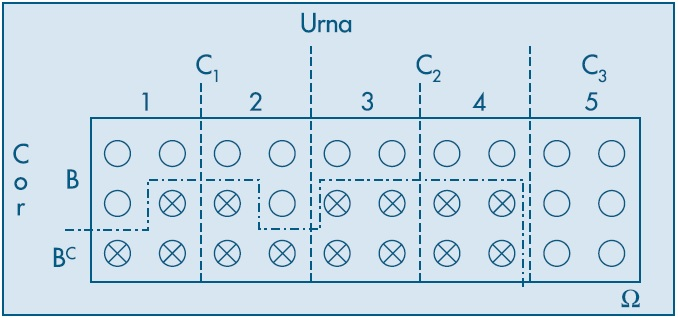
\includegraphics[height=0.3\textwidth,width=15cm]{Figuras/ex5_14}
    %\caption{Exemplo de Histogramas para dados transformados (\cite{Morettin09}).}
    %\label{Fig101_ex}
    \end{figure}
  
\end{frame}


\begin{frame}{}
\frametitle{}
\begin{block}{}
\justifying
Queremos encontrar $P(C_3|B),$ sabendo que
\begin{align*}
P(C_{1})&=2/5,\ P(B|C_{1})=1/2\\
P(C_{2})&=2/5,\ P(B|C_{2})=1/3\\
P(C_{3})&=1/5,\ P(B|C_{3})=1\\
\end{align*}
Da definição de probabilidade condicional, temos
$$P(C_{3}|B)=\dfrac{P(C_{3}\cap B)}{P(B)}=\dfrac{P(C_{3})P(B|C_{3})}{P(B)}$$
\end{block}
\end{frame}

\begin{frame}{}
\frametitle{}
\begin{block}{}
\justifying
Precisamos encontrar o valor de $P(B),$ já que o numerador é conhecido. Como C1,
C2 e C3 são eventos mutuamente exclusivos, e reunidos formam o espaço amostral
completo, podemos decompor o evento B na reunião de três outros, também mutuamente
exclusivos, como $B=(C_{1}\cap B)\cup (C_{2}\cap B)\cup (C_{3}\cap B),$ então:
\begin{align*}
P(B)&=P(C_{1}\cap B)+P(C_{2}\cap B)+P(C_{3}\cap B)\\
&=P(C_{1})P(B|C_{1})+P(C_{2})P(B|C_{2})+P(C_{3})P(B|C_{3})\\
&=\dfrac{2}{5}\times \dfrac{1}{2}+\dfrac{2}{5}\times \dfrac{1}{3}+\dfrac{1}{5}\times 1\\
&=\dfrac{8}{15}
\end{align*}
\end{block}
\end{frame}

\begin{frame}{}
\frametitle{}
\begin{block}{}
\justifying
Logo, 
\begin{align}
P(C_{3}|B)&=\dfrac{P(C_{3})P(B|C_{3})}{P(B)}\\
&=\dfrac{1/5 \times 1}{8/15}\\
&=\dfrac{3}{8}
\end{align}
\end{block}
\end{frame}

% \begin{frame}{}
% \frametitle{}
% \begin{block}{}
% \justifying
% 
% 
% \end{block}
% \end{frame}
% 
% \begin{frame}{}
% \frametitle{}
% \begin{block}{}
% \justifying
% 
% 
% \end{block}
% \end{frame}
% 
% \begin{frame}{}
% \frametitle{}
% \begin{block}{}
% \justifying
% 
% 
% \end{block}
% \end{frame}
% 
% \begin{frame}{}
% \frametitle{}
% \begin{block}{}
% \justifying
% 
% 
% \end{block}
% \end{frame}
% 
% \begin{frame}{}
% \frametitle{}
% \begin{block}{}
% \justifying
% 
% 
% \end{block}
% \end{frame}
% 
% 
% \begin{frame}{}
% \frametitle{}
% \begin{block}{}
% \justifying
% 
% 
% \end{block}
% \end{frame}
% 
% \begin{frame}{}
% \frametitle{}
% \begin{block}{}
% \justifying
% 
% 
% \end{block}
% \end{frame}
% 
% \begin{frame}{}
% \frametitle{}
% \begin{block}{}
% \justifying
% 
% 
% \end{block}
% \end{frame}
% 
% \begin{frame}{}
% \frametitle{}
% \begin{block}{}
% \justifying
% 
% 
% \end{block}
% \end{frame}
% 
% \begin{frame}{}
% \frametitle{}
% \begin{block}{}
% \justifying
% 
% 
% \end{block}
% \end{frame}
% 
% \begin{frame}{}
% \frametitle{}
% \begin{block}{}
% \justifying
% 
% 
% \end{block}
% \end{frame}
% 
% \begin{frame}{}
% \frametitle{}
% \begin{block}{}
% \justifying
% 
% 
% \end{block}
% \end{frame}
% 
% \begin{frame}{}
% \frametitle{}
% \begin{block}{}
% \justifying
% 
% 
% \end{block}
% \end{frame}
% 
% 
% \begin{frame}{}
% \frametitle{}
% \begin{block}{}
% \justifying
% 
% 
% \end{block}
% \end{frame}
% 
% \begin{frame}{}
% \frametitle{}
% \begin{block}{}
% \justifying
% 
% 
% \end{block}
% \end{frame}
% 
% \begin{frame}{}
% \frametitle{}
% \begin{block}{}
% \justifying
% 
% 
% \end{block}
% \end{frame}
% 
% \begin{frame}{}
% \frametitle{}
% \begin{block}{}
% \justifying
% 
% 
% \end{block}
% \end{frame}
% 
% \begin{frame}{}
% \frametitle{}
% \begin{block}{}
% \justifying
% 
% 
% \end{block}
% \end{frame}
% 
% \begin{frame}{}
% \frametitle{}
% \begin{block}{}
% \justifying
% 
% 
% \end{block}
% \end{frame}
% 
% \begin{frame}{}
% \frametitle{}
% \begin{block}{}
% \justifying
% 
% 
% \end{block}
% \end{frame}
% 
% \begin{frame}{}
% \frametitle{}
% \begin{block}{}
% \justifying
% 
% 
% \end{block}
% \end{frame}
% 
% 
% \begin{frame}{}
% \frametitle{}
% \begin{block}{}
% \justifying
% 
% 
% \end{block}
% \end{frame}
% 
% \begin{frame}{}
% \frametitle{}
% \begin{block}{}
% \justifying
% 
% 
% \end{block}
% \end{frame}
% 
% \begin{frame}{}
% \frametitle{}
% \begin{block}{}
% \justifying
% 
% 
% \end{block}
% \end{frame}
% 
% \begin{frame}{}
% \frametitle{}
% \begin{block}{}
% \justifying
% 
% 
% \end{block}
% \end{frame}
% 
% \begin{frame}{}
% \frametitle{}
% \begin{block}{}
% \justifying
% 
% 
% \end{block}
% \end{frame}
% 
% \begin{frame}{}
% \frametitle{}
% \begin{block}{}
% \justifying
% 
% 
% \end{block}
% \end{frame}
% 
% \begin{frame}{}
% \frametitle{}
% \begin{block}{}
% \justifying
% 
% 
% \end{block}
% \end{frame}
% 
% \begin{frame}{}
% \frametitle{}
% \begin{block}{}
% \justifying
% 
% 
% \end{block}
% \end{frame}
% 
% 
% \begin{frame}{}
% \frametitle{}
% \begin{block}{}
% \justifying
% 
% 
% \end{block}
% \end{frame}
% 
% \begin{frame}{}
% \frametitle{}
% \begin{block}{}
% \justifying
% 
% 
% \end{block}
% \end{frame}
% 
% \begin{frame}{}
% \frametitle{}
% \begin{block}{}
% \justifying
% 
% 
% \end{block}
% \end{frame}
% 
% \begin{frame}{}
% \frametitle{}
% \begin{block}{}
% \justifying
% 
% 
% \end{block}
% \end{frame}
% 
% \begin{frame}{}
% \frametitle{}
% \begin{block}{}
% \justifying
% 
% 
% \end{block}
% \end{frame}
% 
% \begin{frame}{}
% \frametitle{}
% \begin{block}{}
% \justifying
% 
% 
% \end{block}
% \end{frame}
% 
% \begin{frame}{}
% \frametitle{}
% \begin{block}{}
% \justifying
% 
% 
% \end{block}
% \end{frame}
% 
% \begin{frame}{}
% \frametitle{}
% \begin{block}{}
% \justifying
% 
% 
% \end{block}
% \end{frame}
% 
% 
% \begin{frame}{}
% \frametitle{}
% \begin{block}{}
% \justifying
% 
% 
% \end{block}
% \end{frame}
% 
% \begin{frame}{}
% \frametitle{}
% \begin{block}{}
% \justifying
% 
% 
% \end{block}
% \end{frame}
% 
% \begin{frame}{}
% \frametitle{}
% \begin{block}{}
% \justifying
% 
% 
% \end{block}
% \end{frame}
% 
% \begin{frame}{}
% \frametitle{}
% \begin{block}{}
% \justifying
% 
% 
% \end{block}
% \end{frame}
% 
% \begin{frame}{}
% \frametitle{}
% \begin{block}{}
% \justifying
% 
% 
% \end{block}
% \end{frame}
% 
% \begin{frame}{}
% \frametitle{}
% \begin{block}{}
% \justifying
% 
% 
% \end{block}
% \end{frame}
% 
% \begin{frame}{}
% \frametitle{}
% \begin{block}{}
% \justifying
% 
% 
% \end{block}
% \end{frame}
% 
% \begin{frame}{}
% \frametitle{}
% \begin{block}{}
% \justifying
% 
% 
% \end{block}
% \end{frame}
% 
% 
% \begin{frame}{}
% \frametitle{}
% \begin{block}{}
% \justifying
% 
% 
% \end{block}
% \end{frame}
% 
% \begin{frame}{}
% \frametitle{}
% \begin{block}{}
% \justifying
% 
% 
% \end{block}
% \end{frame}
% 
% \begin{frame}{}
% \frametitle{}
% \begin{block}{}
% \justifying
% 
% 
% \end{block}
% \end{frame}
% 
% \begin{frame}{}
% \frametitle{}
% \begin{block}{}
% \justifying
% 
% 
% \end{block}
% \end{frame}
% 
% \begin{frame}{}
% \frametitle{}
% \begin{block}{}
% \justifying
% 
% 
% \end{block}
% \end{frame}
% 
% \begin{frame}{}
% \frametitle{}
% \begin{block}{}
% \justifying
% 
% 
% \end{block}
% \end{frame}
% 
% \begin{frame}{}
% \frametitle{}
% \begin{block}{}
% \justifying
% 
% 
% \end{block}
% \end{frame}
% 
% \begin{frame}{}
% \frametitle{}
% \begin{block}{}
% \justifying
% 
% 
% \end{block}
% \end{frame}
% 
% 
% \begin{frame}{}
% \frametitle{}
% \begin{block}{}
% \justifying
% 
% 
% \end{block}
% \end{frame}
% 
% \begin{frame}{}
% \frametitle{}
% \begin{block}{}
% \justifying
% 
% 
% \end{block}
% \end{frame}
% 
% \begin{frame}{}
% \frametitle{}
% \begin{block}{}
% \justifying
% 
% 
% \end{block}
% \end{frame}
% 
% \begin{frame}{}
% \frametitle{}
% \begin{block}{}
% \justifying
% 
% 
% \end{block}
% \end{frame}
% 
% \begin{frame}{}
% \frametitle{}
% \begin{block}{}
% \justifying
% 
% 
% \end{block}
% \end{frame}
% 
% \begin{frame}{}
% \frametitle{}
% \begin{block}{}
% \justifying
% 
% 
% \end{block}
% \end{frame}
% 
% \begin{frame}{}
% \frametitle{}
% \begin{block}{}
% \justifying
% 
% 
% \end{block}
% \end{frame}
% 
% \begin{frame}{}
% \frametitle{}
% \begin{block}{}
% \justifying
% 
% 
% \end{block}
% \end{frame}
% 
% 
% \begin{frame}{}
% \frametitle{}
% \begin{block}{}
% \justifying
% 
% 
% \end{block}
% \end{frame}
% 
% \begin{frame}{}
% \frametitle{}
% \begin{block}{}
% \justifying
% 
% 
% \end{block}
% \end{frame}
% 
% \begin{frame}{}
% \frametitle{}
% \begin{block}{}
% \justifying
% 
% 
% \end{block}
% \end{frame}
% 
% \begin{frame}{}
% \frametitle{}
% \begin{block}{}
% \justifying
% 
% 
% \end{block}
% \end{frame}
% 
% \begin{frame}{}
% \frametitle{}
% \begin{block}{}
% \justifying
% 
% 
% \end{block}
% \end{frame}
% 
% \begin{frame}{}
% \frametitle{}
% \begin{block}{}
% \justifying
% 
% 
% \end{block}
% \end{frame}
% 
% \begin{frame}{}
% \frametitle{}
% \begin{block}{}
% \justifying
% 
% 
% \end{block}
% \end{frame}
% 
% \begin{frame}{}
% \frametitle{}
% \begin{block}{}
% \justifying
% 
% 
% \end{block}
% \end{frame}

\begin{frame}{}
\frametitle{Referências Bibliográficas}
\bibliography{bibliografia}
\end{frame}
\end{document}
